\documentclass[12pt,a4paper,notitlepage]{report}
\usepackage[utf8]{inputenc}
\usepackage[polish]{babel}
\usepackage[T1]{fontenc}
\usepackage[top=2cm, bottom=2cm, left=3cm, right=3cm]{geometry}
\usepackage[dvipsnames]{xcolor}
\definecolor{Red}{RGB}{255,36,0}
\usepackage{changepage}
\usepackage{indentfirst}
\usepackage{color}
\usepackage{graphicx}
\definecolor{bluekeywords}{rgb}{0.13,0.13,1}
\definecolor{greencomments}{rgb}{0,0.5,0}
\definecolor{redstrings}{rgb}{0.9,0,0}
\usepackage{listings}
\lstset{language=[Sharp]C,
  showspaces=false,
  showtabs=false,
  breaklines=true,
  showstringspaces=false,
  breakatwhitespace=true,
  escapeinside={(*@}{@*)},
  commentstyle=\color{greencomments},
  keywordstyle=\color{bluekeywords},
  stringstyle=\color{redstrings},
  basicstyle=\ttfamily,
  extendedchars=true
}
\makeatletter
\newcommand{\linia}{\rule{\linewidth}{0.4mm}}
\renewcommand{\maketitle}{\begin{titlepage}
    \vspace*{1cm}
    \begin{center}\small
    Politechnika Wrocławska\\
    Wydział Elektroniki\\
    Urządzenia Peryferyjne 
    \end{center}
    \vspace{4.5cm}
    \noindent\linia
    \begin{center}
      \LARGE \textsc{\@title}
         \end{center}
     \linia
    \vspace{0.5cm}
    \begin{flushright}
    \begin{minipage}{6cm}
    
     \vspace{4cm}
     \textit{\small Termin zajęć:}\\
     \normalsize \textsc{Wtorek TN 7:30} \par
	\vspace{0.3cm}    
    \textit{\small Autorzy:}\\
    \normalsize \textsc{\@author} \par
     \vspace{0.3cm}
        Prowadzący: \\ dr inż. Tomasz Walkowiak

    \end{minipage}
    \vspace{1cm}
     {\small }\\
       
     \end{flushright}
    \vspace*{\stretch{3}}
    \begin{center}
    \@date
    \end{center}
  \end{titlepage}%
}
\makeatother
\author{ Jakub Chmiel  235028 \\ Tomasz Cieślar 235652}
\title{Drukowanie kodów paskowych}
\begin{document}
\maketitle

\newpage
\tableofcontents
\newpage
\renewcommand*\thesection{\arabic{section}}
\section{Cel ćwiczenia}
\begin{enumerate}
\item Napisać program do drukowania kodów kreskowych w standardzie EAN13 wykorzystujac drukarkę mozaikową:
\begin{itemize}
\item wprowadzić kod (cyfrowo - bez ostatniej cyfry) 
\item wygenerować kod jako plik graficzny
\item wydrukować cyfry kodu
\end{itemize}
\end{enumerate}

\section{Wstęp}
Kod kreskowy – graficzna reprezentacja informacji poprzez kombinację ciemnych i jasnych elementów, ustaloną według symboliki reguł opisujących budowę kodu, (np. jego wymiary, zbiór kodowanych znaków, algorytm obliczania cyfry kontrolnej i inne) danego kodu. Kod kreskowy przeznaczony jest dla czytników elektronicznych. Ma na celu umożliwienie automatycznego odczytywania informacji. Głównym zastosowaniem kodu kreskowego jest automatyczna identyfikacja produktów w szeroko pojętej logistyce.
\\
\indent EAN (ang. European Article Number – Europejski Kod Towarowy) – rodzina kodów kreskowych (symbolika) wprowadzona w 1976 roku przez stowarzyszenie European Article Numbering. Kod został opracowany na podstawie opracowanego wcześniej w USA i Kanadziekodu UPC. Symbolika została zaimplementowana w globalnym systemie GS1. Jest to kod ciągły, numeryczny, modularny, samosprawdzalny z dodatkową obowiązkową cyfrą kontrolną. Kod wymaga stosunkowo wysokiej precyzji wydruku, stąd nie może być stosowany na niskiej jakości papierze (np. kartonie) oraz wymaga w miarę dobrej jakości drukarek.
\\
\indent Kod posiada stałą długość. Stosuje się dwie wersje kodu:
\begin{itemize}
\item EAN-13 – zawiera 12 cyfr danych i jedną cyfrę kontrolną
\item EAN-8 – zawiera 7 cyfr danych i jedną cyfrę kontrolną
\end{itemize}
\indent W Europie symbolika ta jest powszechnie wykorzystywana do znakowania opakowań jednostkowych oraz zbiorczych (zarówno EAN-8, jak i EAN-13). Wersję EAN-13 wykorzystuje się również m.in. do kodowania numerów ISBN, ISMN czy ISSN.
Kod EAN-8 przeznaczono dla małych opakowań, na których nie zmieściłby się kod EAN-13. Jednakże ze względu na wyczerpywanie się puli kodów EAN-13 przydzielonych danemu producentowi, wielu z nich stosuje indywidualnie przydzielane kody EAN-8 na dużych opakowaniach.
\\
\indent Przy oznaczaniu opakowań jednostkowych w kodzie EAN-13 wyróżnia się cztery grupy:
\begin{itemize}
\item Kod systemowy obejmujący pierwsze dwie lub trzy cyfry. Zwykle oznaczają one kod kraju (np. 590 – Polska), z wyjątkiem oznaczeń rozpoczynających się od cyfry 2 – tzw. kodów wagowych, takimi kodami oznaczane są produkty o zmiennej masie i rozmiarach, zazwyczaj konfekcjonowane w sklepach. Kod systemowy nie oznacza jednak kraju pochodzenia towaru lub przedsiębiorstwa, lecz jedynie numer organizacji krajowej, w której dany produkt jest zarejestrowany. W przypadku kodowania numerów ISSN w kodzie występuje przedrostek 977, natomiast 978 lub 979 dla ISBN (w wersji dziesięciocyfrowej) i 979 dla ISMN.
\item Kod producenta składający się z czterech, pięciu lub sześciu cyfr, w zależności od długości kodu systemowego.
\item Kod produktu o długości zależnej od długości kodu systemowego i kodu producenta.
\item Cyfra kontrolna.
\end{itemize}
\section{Założenia projektowe}
\begin{itemize}
\item Program był pisany w języku C\texttt{\#}.
\item Na komputerze, na którym uruchamiany był program zainstalowano system operacyjny Windows 10 w wersji 64-bitowej.
\item Kod kreskowy należało wygenerować bez użycia gotowych bibliotek
\end{itemize}

\section{Wykorzystane narzędzia}
\begin{itemize}
\item Windows Forms - API do implementacji interfejsu graficznego dla platformy .NET.
\end{itemize}
\begin{adjustwidth}{0pt}{-50pt}
\section{Implementacja programu}
\subsection{Interfejs aplikacji}
\begin{center}
\noindent 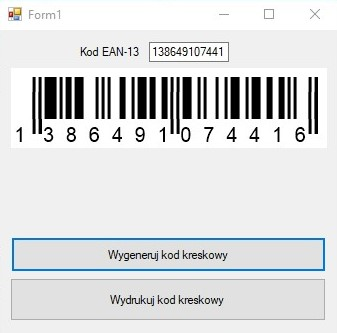
\includegraphics[scale=0.85]{okno}
\\
\begin{normalsize}
\textit{Rysunek 1. Interfejs aplikacji}
\end{normalsize}
\end{center}
\newpage
\subsection{Kod źródłowy}
\begin{lstlisting}
using [...]

namespace UP_Kody
{
    public partial class Form1 : Form
    {
    	//Tablice przechowujace schematy kodowania EAN-13
        private string[] odd = { "0001101", "0011001", "0010011", "0111101", "0100011", "0110001", "0101111", "0111011", "0110111", "0001011" };
        private string[] even = { "0100111", "0110011", "0011011", "0100001", "0011101", "0111001", "0000101", "0010001", "0001001", "0010111" };
        private string[] parity = { "oooooo", "ooeoee", "ooeeoe", "ooeeeo", "oeooee", "oeeooe", "oeeeoo", "oeoeoe", "oeoeeo", "oeeoeo" };
        private string[] right = { "1110010", "1100110", "1101100", "1000010", "1011100", "1001110", "1010000", "1000100", "1001000", "1110100" };

        public Form1()
        {
            InitializeComponent();
            maskedTextBox1.Select();
        }
        private void button2_Click(object sender, EventArgs e)
        {
            PrintDocument printDocument = new PrintDocument();
            printDocument.PrintPage += PrintGeneratedBarcode;
            printDocument.Print();
        }

        private static void PrintGeneratedBarcode(object o, PrintPageEventArgs e)
        {
            System.Drawing.Image image = System.Drawing.Image. FromFile(@"C:\Users\DELl\Desktop\myimage.jpg");
            Point loc = new Point(100, 100);
            e.Graphics.DrawImage(image, loc);
        }

        private void button3_Click(object sender, EventArgs e)
        {
            var eanCode = maskedTextBox1.Text;
            var controlSum = 0;
            //Wyliczanie sumy kontrolnej, na zmiane *1 i *3
            for (var i = 0; i < eanCode.Length - 1; i += 2)
            {
                controlSum += Int32.Parse(eanCode[i] + "");
                controlSum += 3 * Int32.Parse(eanCode[i + 1] + "");
            }
            //Reszta z dzielenia przez 10
            controlSum = controlSum % 10;
            controlSum = 10 - controlSum;
            if (controlSum == 10)
            {
                controlSum = 0;
            }
            //StringBuilder przechowujacy 0 i 1 kodu kreskowego
            var barcode = new StringBuilder();
            //Pierwszy guard
            barcode.Append("101");
            //Przepisujemy pierwsza cyfre
            var first = Convert.ToInt32(maskedTextBox1.Text[0]) - 48;
            var scheme = parity[first];
            //Kodujemy zgodnie z maska odd/even
            for (var i = 1; i < 7; i++)
            {
                if (scheme[i - 1] == 'o')
                {
                    barcode.Append(odd[Convert. ToInt32(maskedTextBox1.Text[i]) - 48]);
                }
                if (scheme[i - 1] == 'e')
                {
                    barcode.Append(even[Convert. ToInt32(maskedTextBox1.Text[i]) - 48]);
                }
            }
            //Drugi guard
            barcode.Append("01010");
            //Kodujemy kolejne cyfry zgodnie z tablica right
            for (var i = 7; i < 12; i++)
            {
                barcode.Append(right[Convert. ToInt32(maskedTextBox1.Text[i]) - 48]);
            }
			//Dodajemy dume kontrolna
            barcode.Append(right[controlSum]);
			//Ostatni guard
            barcode.Append("101");
			//Czcionki do grafiki
            Font barCodeF = new Font("Free 3 of 9", 45, FontStyle.Regular, GraphicsUnit.Pixel);
            Font plainTextF = new Font("Arial", 20, FontStyle.Regular, GraphicsUnit.Pixel);

            Bitmap bmp = new Bitmap(1, 1);
            Graphics graphics = Graphics.FromImage(bmp);

            int barCodewidth = (int)graphics.MeasureString(maskedTextBox1.Text, barCodeF).Width + 100;
            int barCodeHeight = (int)graphics.MeasureString(maskedTextBox1.Text, barCodeF).Height;

            int plainTextWidth = (int)graphics.MeasureString(maskedTextBox1.Text, plainTextF).Width + 100;
            int plainTextHeight = (int)graphics.MeasureString(maskedTextBox1.Text, plainTextF).Height;

            
                bmp = new Bitmap(bmp,
                                 new Size(plainTextWidth, barCodeHeight + plainTextHeight));
            }
            graphics = Graphics.FromImage(bmp);

            graphics.Clear(Color.White);
            graphics.SmoothingMode = SmoothingMode.AntiAlias;
            graphics.TextRenderingHint = TextRenderingHint.AntiAlias;

            for (var i = 0; i < 95; i++)
            {
                if (i < 3 || (i > 45 && i < 50) || i > 91)
                {
                    if (barcode[i] == '0')
                    {
                        graphics.DrawString("|",
                            barCodeF,
                            new SolidBrush(Color.White),
                            10 + i * 3,
                            15);
                    }
                    else
                    {
                        graphics.DrawString("|",
                            barCodeF,
                            new SolidBrush(Color.Black),
                            10 + i * 3,
                            15);
                    }
                }
                if (barcode[i] == '0')
                {
                    graphics.DrawString("|",
                        barCodeF,
                        new SolidBrush(Color.White),
                        10 + i * 3,
                        0);
                }
                else
                {
                    graphics.DrawString("|",
                        barCodeF,
                        new SolidBrush(Color.Black),
                        10 + i * 3,
                        0);
                }
            }
            var numbers = new StringBuilder();
            numbers.Append(maskedTextBox1.Text[0] - 48);
            numbers.Append("   ");
            for (var i = 1; i < 7; i++)
            {
                numbers.Append(Convert.ToInt32 (maskedTextBox1.Text[i]) - 48);
                numbers.Append("  ");
            }
            numbers.Append("");
            for (var i = 7; i < 12; i++)
            {
                numbers.Append(Convert.ToInt32 (maskedTextBox1.Text[i]) - 48);
                numbers.Append("  ");
            }
            numbers.Append(controlSum);
            graphics.DrawString(Convert.ToString(numbers),
                        plainTextF,
                        new SolidBrush(Color.Black),
                        0,
                        barCodeHeight);

            bmp.Save(@"C:\Users\DELl\Desktop\myimage.jpg", ImageFormat.Jpeg);
            pictureBox1.Image = bmp;
        }
    }

\end{lstlisting}

\end{adjustwidth}
\newpage
\section{Wnioski}
Nie udało nam się wykonać całości zadania, ponieważ nie potrafiliśmy wydrukować kodu kreskowego, używając drukarki mozaikowej. Pomyślnie wykonaliśmy natomiast generowanie pliku graficznego kodu kreskowego.
\section{Bibliografia}
\begin{itemize}
\item International Article Number:
\\
$https://en.wikipedia.org/wiki/International\_Article\_Number$
\item Encoding EAN-13:
\\
$http://www.gomaro.ch/Specifications/EAN13e.htm$
\end{itemize}

\end{document}